\section{Reproducibility}
\only<article>{
  One of the main problems in science is reproducibility: when we are trying to draw conclusions from one specific data set, it is easy to make a mistake. For that reason, the scientific process requires us to use our conclusions to make testable predictions, and then test those predictions with new experiments. The same thing can be done in when dealing purely with data, by making sure we use some of the data as input to the algorithm, and other data to measure the quality of the algorithm itself. In the following, we assume we have some algorithm $\alg : \Datasets \to \CY$, where $\Datasets$ is the universe of possible input data and $\CY$ the possible outputs, e.g. all possible classification rules. We also assume the existence of some quality measure $U$.
}

\begin{frame}
  \frametitle{The decision process in data science}
    \centering
    \begin{tikzpicture}[line width=2pt]
    \node[select] at (0,0) (bt) {learning algorithm};
    \node[select] at (0,2) (at) {data collection};
    \node[RV] at (3,-2) (training) {training};
    \node[RV] at (7,2) (holdout) {holdout};
    \draw[blue,->] (at) -- (training);
    \draw[blue,->] (at) -- (holdout);
    \node[RV] at (4,0) (bt2) {model};
    \draw[red,->] (at) -- (bt2);
    \draw[red,->] (bt) -- (bt2);
    \draw[red,->] (training) -- (bt2);
    \node[utility] at (8,0) (rt2) {result};
    \draw[red,->] (bt2) -- (rt2);
    \draw[red,->] (holdout) -- (rt2);
  \end{tikzpicture}
\end{frame}

\begin{frame}
  \frametitle{Holdout sets}
  \begin{itemize}
  \item Original data $\Data$, e.g. $\Data = (x_1, \ldots, x_T)$.
  \item Training data $\Training \subset \Data$, e.g. $\Training = x_1, \ldots, x_n$, $n < T$.
  \item Holdout data $\Holdout = D \setminus \Training$, used to measure the quality of the result.
  \item Get algorithm output $y = \alg(\Training)$.
  \item Calculate quality of output $U(y, \Holdout)$
  \end{itemize}
  \only<article>{
    As typically algorithms are maximising the quality metric on the training data, 
    \[
      \alg(\Training) = \argmax_y U(y, \Training)
    \]
    we typically obtain a biased estimate.
  }
\end{frame}

\begin{frame}
  \frametitle{Bootstrapping}
  Bootstrapping is a general technique that can be used to.
  \begin{itemize}
  \item Estimate the sensitivity of $\alg$ to the data $x$
  \item Obtain a distribution of estimates $y$ from $\alg$ and the data $x$.
  \end{itemize}
  \begin{block}{Bootstrapping}
    \begin{itemize}
    \item \textbf{Input} Training data $\Training$, number of samples $k$.
    \item \textbf{For} $i = 1, \ldots, k$
    \item \quad $\Data^{(i)} = \textrm{Bootstrap}(\Training)$
    \item \quad $y_i = \alg(\Data^{(i)})$
    \item \textbf{return} $\{y_1, \ldots, y_i\}$.
    \end{itemize}
    where  $\textrm{Bootstrap}(\Training)$ samples with replacement $|\Training|$ points.
  \end{block}

\end{frame}
\only<article>{
  In general, it is worthwhile to have some indication of how certain we should be about our prediction. Bayesian inference offers a principled way to do this.
}

\begin{frame}
  \frametitle{Finding important features}
  \only<article>{What features can best explain a difference between two classes?}
\end{frame}

\begin{frame}
  \frametitle{Compare the average difference of features between two classes.}
\end{frame}

\begin{frame}
  \frametitle{Holdout sets}
  \only<article>{
    Your typical algorithm $\alg$ will take some data $x$ and produce some output $y$. Before even trying to interpret this $y$, you must consider first how the $y$ 
  }
  \only<presentation>{
    \begin{itemize}
    \item
    \end{itemize}
  }
\end{frame}

\begin{frame}
  \frametitle{Bootstrapping}
  \only<article>{Bootstrapping is a general technique that can be used to }
  \begin{itemize}
  \item Estimate the sensitivity of $\alg$ to the data $x$
  \item Obtain a distribution of estimates $y$ from $\alg$ and the data $x$.
  \end{itemize}
\end{frame}

\section{Reproducibility}

\begin{frame}
  \frametitle{Reproducibility}
  \begin{itemize}
  \item We use our machine learning algorithm $\alg$ on some data $x$ and get result $y = \alg(x)$.
  \item What does this result mean?
  \item Would we get the same result again?
  \end{itemize}
  \only<2>{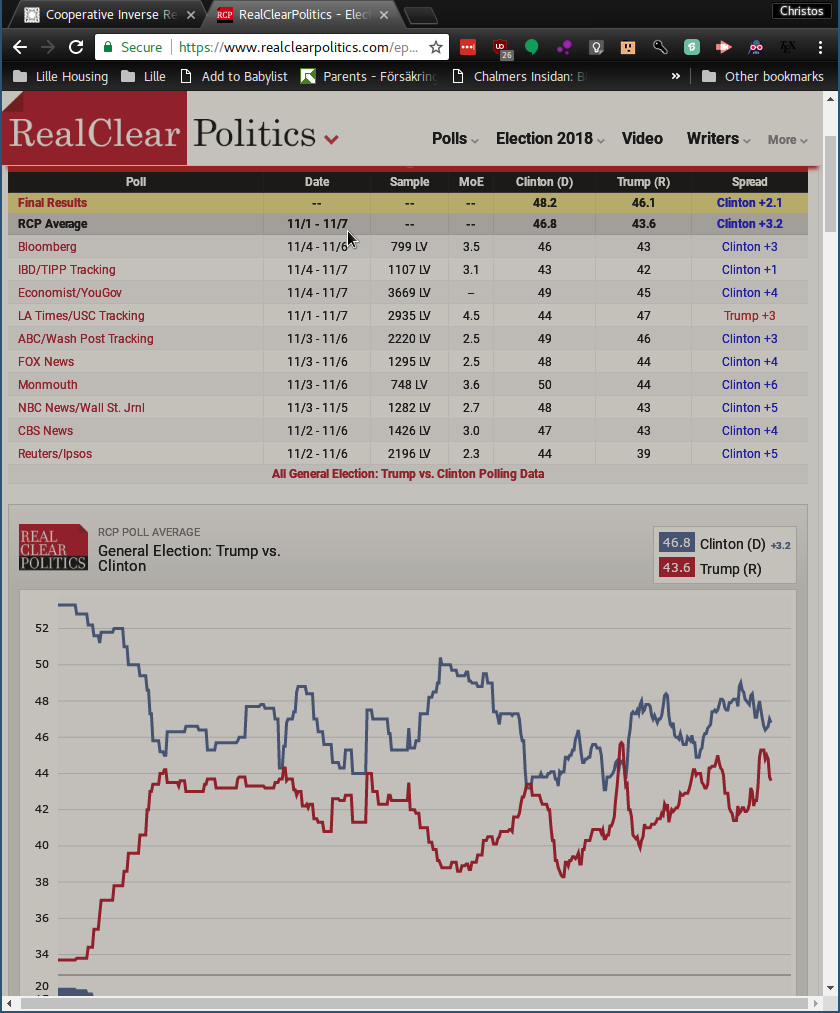
\includegraphics[width=\textwidth]{../figures/2016-election}}
\end{frame}

\subsection{Confidence intervals and $p$-values}
\begin{frame}
  \frametitle{The fallacy of $p$-values}
  \only<article>{A $p$-value has a uniform distribution under the null hypothesis. More precisely,let $x$ is our data and $H_0$ is our null hypothesis. If $H_0$ is true then $x \sim P_0$. Let}
  \[
    f(x) \tag{$p$-statistic}
  \]
  \only<article>{be a statistic on the data designed to have the property:}
  \[
    P_0(\cset{x}{f(x) \leq p}) = p.
  \]
  \only<article>{This ensures that the probability of rejecting the null hypothesis when it is true is actually $p$. But note that this is the definition of the uniform distribution, so $f(x)$ has a uniform distribution under $H_0$. Hence the value of $f(x)$ itself is uninformative. In theory we should simply choose $p$ before seeing the data and just accept or reject based on whether $f(x) \leq p$. However nobody does that in practice, meaning that $p$-values are used incorrectly. Better not to use them at all.}
\end{frame}


\begin{frame}
  \frametitle{Confidence intervals}
  \only<article>{Similarly, a confidence interval $I$ tells us the probability of an underlying value $\theta$ to be estimated being in $\theta \in I$, if our modelling assumption is correct.}
  \begin{block}[Confidence interval under a model $\mu$]
    \only<article>{
      The interval $I(\delta)$ for an estimator $\hat{\theta}$ of a parameter $\theta$ from data $x$ under the modelling assumptions $\mu$ is simply a set in $\Theta$ such that the true parameter lies in $I(\delta)$ with probability $1 - \delta$, i.e.
    }
    \[
      \Pr_\mu(\hat{\theta} \in I(\theta, \delta)) \geq 1 - \delta.
    \]
  \end{block}
  This is a property of the estimator $\hat{\theta} : \CX \to \Theta$ and tells us \emph{nothing direct} about our specific estimate $\hat{\theta(x)}$. \only<article>{It only tells that if we repeatedly apply this produre, we will only get an estimate outside of the interval a $\delta$-fraction of the time.}
\end{frame}

\subsection{Bayesian credible intervals}


\subsection{Model mismatch}

\subsection{Boot-strapping}

\subsection{Cross-validation}

\subsection{Independent replication}



%%% Local Variables:
%%% mode: latex
%%% TeX-master: "notes"
%%% End:

 